\documentclass{llncs}
\usepackage[utf8]{inputenc}
\usepackage{verbatim}
\usepackage{multicol}
\usepackage{llncsdoc}
\usepackage{amsmath}
\usepackage{amsfonts}
\usepackage{amssymb}
\usepackage{graphicx}
\usepackage{lmodern}
\usepackage{calc}
\usepackage{enumitem}
\usepackage{algpseudocode}
\usepackage{algorithm}
\usepackage{algorithmicx}

\algsetblockdefx[IfContinue]{IfContinue}{IfContinue}
{0}{0pt}
[0]{}
[1]{\textbf{if} #1 \textbf{continue}}

\algrenewcommand\algorithmicrequire{%
  \makebox[\widthof{\textbf{Output:}}][l]{\textbf{Input:}}}
  
 \algrenewcommand\algorithmicensure{%
  \textbf{Output:}}

\usepackage{color}
\usepackage{gnuplottex}
\usepackage{subcaption}
\usepackage{microtype}
\usepackage[normalem]{ulem}
\captionsetup{compatibility=false}
\usepackage{tikz}
\usetikzlibrary{trees,automata,positioning}
\usepackage{booktabs}
\usepackage{gnuplottex}
\usepackage{xparse}
\usepackage{epstopdf}
% For scaling gnuplottex
\ExplSyntaxOn
\DeclareExpandableDocumentCommand{\convertlen}{ O{cm} m }
 {
  \dim_to_unit:nn { #2 } { 1 #1 } cm
 }
\ExplSyntaxOff

%% For lattice figure
% Set the overall layout of the tree
\tikzstyle{level 1}=[level distance=3.0cm, sibling distance=0.6cm]
\tikzstyle{level 2}=[level distance=3.5cm, sibling distance=0.6cm]
\tikzstyle{level 3}=[level distance=3.5cm, sibling distance=0.6cm]

% Define styles for bags and leafs
\tikzstyle{l1} = [rectangle, text width=5em, text centered]
\tikzstyle{l2} = [rectangle, text width=5em, text centered]
\tikzstyle{l3} = [rectangle, text width=5em, text centered]

% only when using asmthm
%\newtheorem{definition}{Definition}
%\newtheorem{theorem}{Theorem}

\author{Micky Faas \and Matthijs van Leeuwen}
\title{VOUW: Geometric Pattern Mining using the MDL Principle}
\institute{Leiden Institute for Advances Computer Science}
\begin{document}

\section{Experiments}

\begin{figure}[t]
\centering
\begin{subfigure}[t]{0.25\textwidth}
\centering
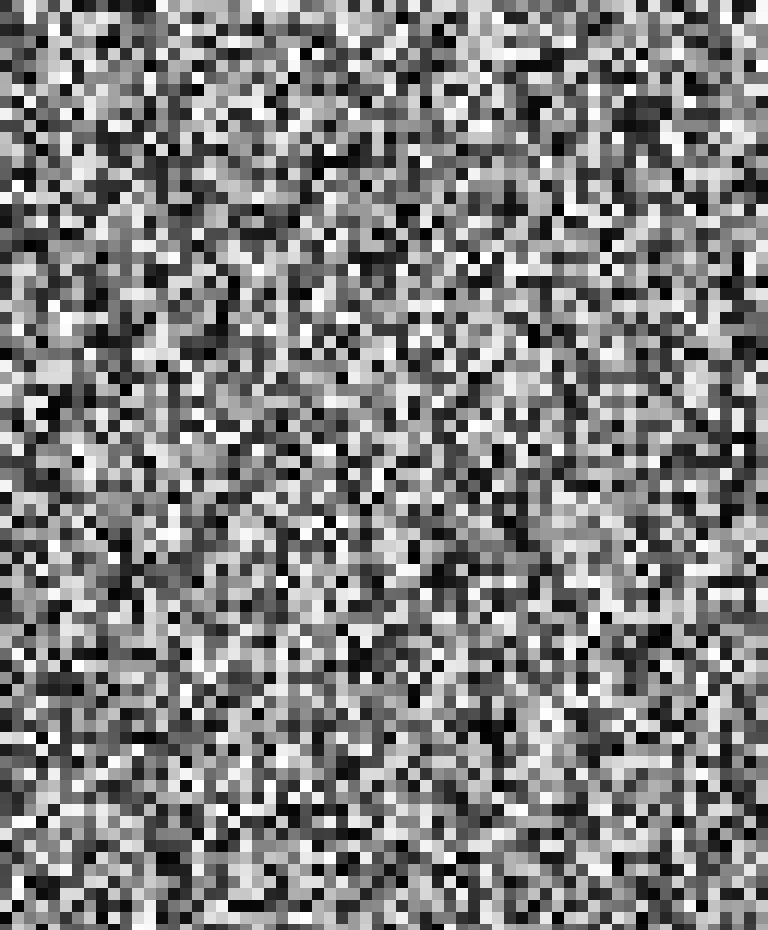
\includegraphics[scale=.88]{img/exp_input_2_cropped.png}
\caption{Generated matrix}
\label{fig:rila}
\end{subfigure}%
~
\begin{subfigure}[t]{0.25\textwidth}
\centering
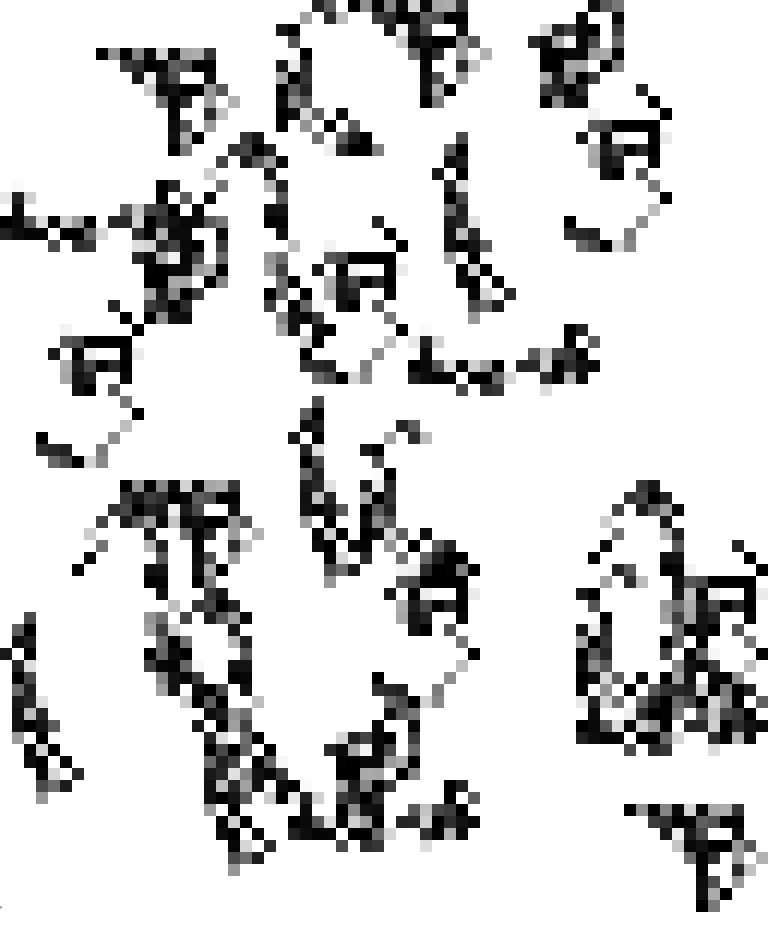
\includegraphics[scale=.88]{img/exp_inputpatterns_2_cropped.png}
\caption{Ground truth}
\label{fig:rilb}
\end{subfigure}%
~
\begin{subfigure}[t]{0.25\textwidth}
\centering
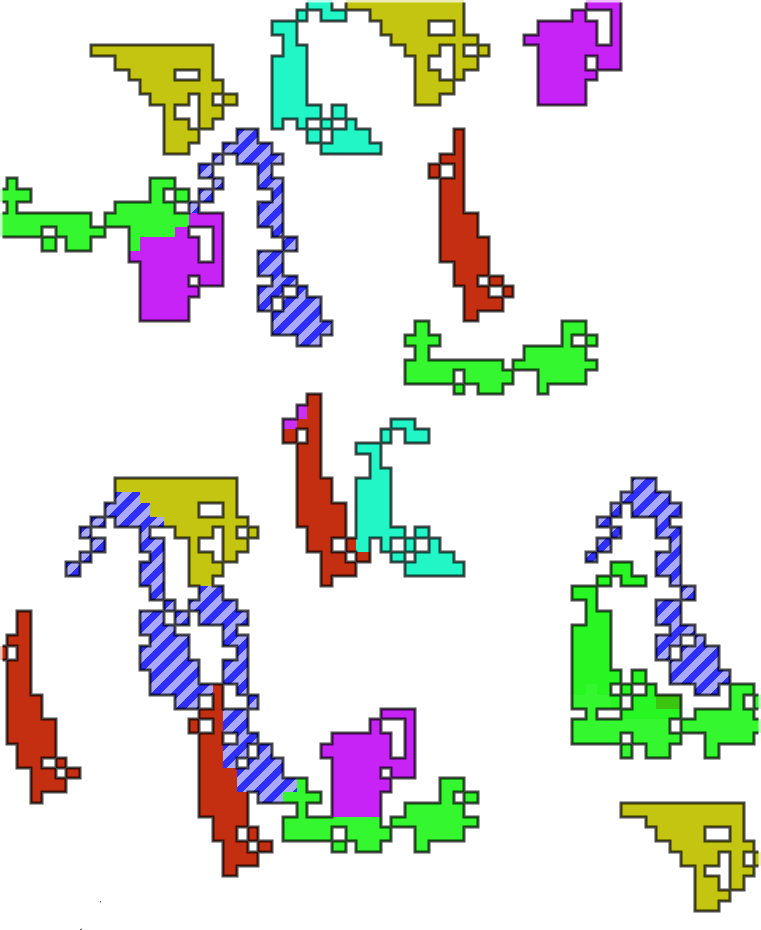
\includegraphics[scale=.88]{img/exp_result_2_cropped.png}
\caption{Found patterns}
\label{fig:rilc}
\end{subfigure}%
~
\begin{subfigure}[t]{0.25\textwidth}
\centering
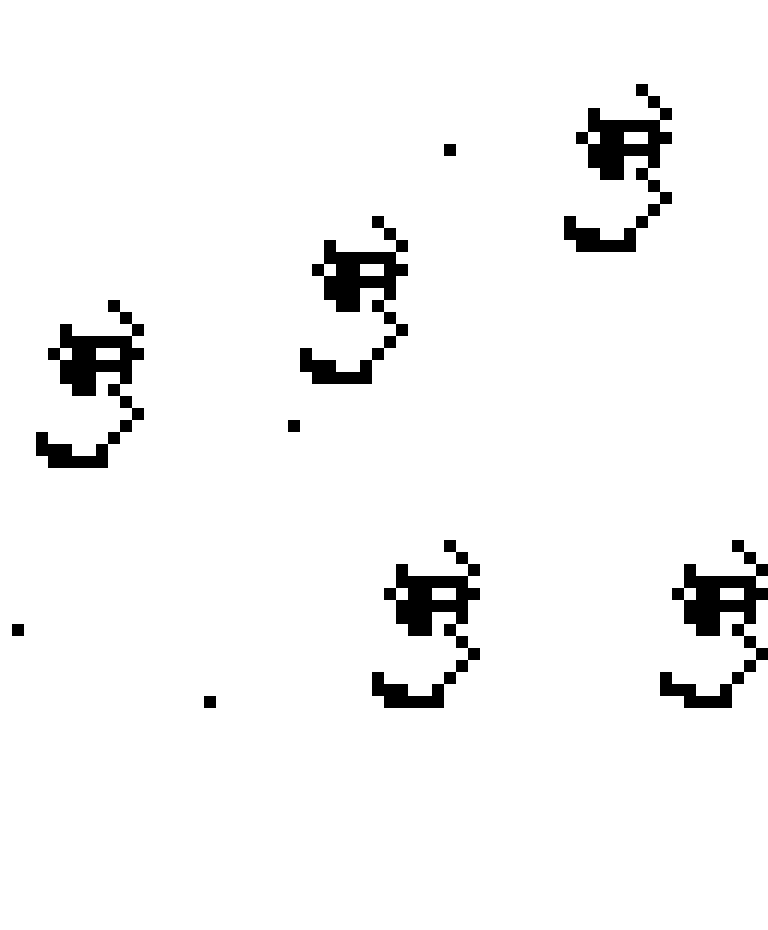
\includegraphics[scale=.88]{img/exp_diff_2_cropped.png}
\caption{Difference}
\label{fig:rild}
\end{subfigure}%
\caption{Synthetic patterns are added to a matrix filled with noise. The difference between the ground truth and the matrix reconstructed by the algorithm is used to compute precision and recall.}
\label{fig:ril}
\end{figure}  

%%
%% The following LaTeX + Gnuplot code generates the two graphs using the gnuplottex package
%% It can be omitted by directly including the pre-baked PDFs as figures
%%

%\begin{comment}
\begin{figure}[t]%
	%\centering%
	\begin{subfigure}[t]{0.5\textwidth}
	%\centering
	\begin{gnuplot}[terminal=epslatex, terminaloptions={color dashed size 6.5cm,5cm font "lmodern,8"}]
		set key box bottom left
		set key width 1.0
		set key height 1.0
		set key spacing 1.1
		set key opaque
		set sample 1000
		set xr [0:.7]
		set yr [.3:1]
		set grid xtics lt 0 ls 0
		set grid ytics lt 0 ls 0
		set xlabel 'Signal-to-noise Ratio'
		set ylabel 'Compression'
		#plot "data/256_snr_vs_prec_n10.txt" w l lc 1 lw 1 t "precision",\
		#	 "data/256_snr_vs_recall_n10.txt" w l lc 2 lw 1 t "recall",\
		#	 "data/256_snr_vs_compr_n10.txt" w l lc 3 lw 1 t "ratio"
		plot "data/output_snr_256.txt" using 4:5 w l lc 1 lw 2.5 t "256",\
  			 "data/output_snr_512.txt" using 4:5 w l lc 2 lw 2.5 t "512",\
  			 "data/output_snr_1024.txt" using 4:5 w l lc 3 lw 2.5 t "1024",\
  			 "data/output_snr_2048.txt" using 4:5 w l lc 4 lw 2.5 t "2048"
	\end{gnuplot}}\
	%\caption{The influence of SNR in the ground truth}
	%\label{fig:snr}
	\end{subfigure}%
	%\vspace{-\baselineskip}
	~
	\begin{subfigure}[t]{0.5\textwidth}
	%\centering
	\begin{gnuplot}[terminal=epslatex, terminaloptions={color dashed size 6.5cm,5cm font "lmodern,8"}]
		set key box bottom right
		set key width 1.0
		set key height 1.0
		set key spacing 1.1
		set key opaque
		set sample 1000
		set xr [0:50]
		set yr [0:1]
		set grid xtics lt 0 ls 0
		set grid ytics lt 0 ls 0
		set xlabel 'Prevalence per Pattern'
		set ylabel 'Recall' offset 1,0,0
		plot "data/usage_test_128.txt" using 1:8 w l lc 1 lw 2.5 t "128",\
			 "data/usage_test_256.txt" using 1:8 w l lc 2 lw 2.5 t "256",\
			 "data/usage_test_512.txt" using 1:8 w l lc 3 lw 2.5 t "512",\
			 "data/usage_test_1024.txt" using 1:8 w l lc 4 lw 2.5 t "1024"
	\end{gnuplot}
	%\vspace{-\baselineskip}
	%\caption{Prevalence versus recall}
	%\label{fig:usage}
	\end{subfigure}
	%\caption{Qualitative results for increasingly large matrices (sizes are squared). }
	\caption{The influence of SNR in the ground truth (left) and prevalence on recall (right)} 
	\label{fig:plots}
\end{figure}
%\end{comment}

%%
%% End of Gnuplottex section
%%

% Begin of proxy graphs from PDF
\begin{comment}
\begin{figure}[t]%
	\begin{subfigure}[t]{0.5\textwidth}
	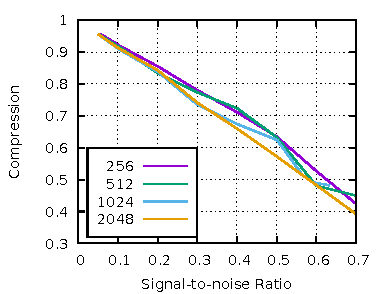
\includegraphics[scale=1]{figures/experiments-gnuplottex-fig1.pdf}
	%\caption{The influence of SNR in the ground truth}
	%\label{fig:snr}

	\end{subfigure}%
	%\vspace{-\baselineskip}
	~
	\begin{subfigure}[t]{0.5\textwidth}
	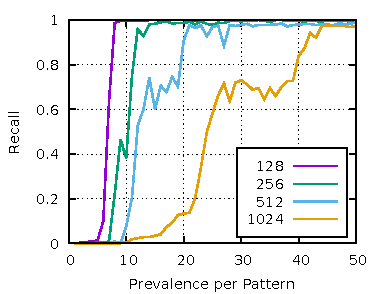
\includegraphics[scale=1]{figures/experiments-gnuplottex-fig2.pdf}
	%\vspace{-\baselineskip}
	%\caption{Prevalence versus recall}
	%\label{fig:usage}
	\end{subfigure}
	\caption{The influence of SNR in the ground truth (left) and prevalence on recall (right).} 
	\label{fig:plots}
\end{figure}
\end{comment}
% End of proxy graphs

To asses Vouw's practical performance we primarily use Ril, a synthetic dataset generator developed for this purpose. Ril utilises random walks to populate a matrix with patterns of a given size and prevalence, up to a specified density, while filling the remainder of the matrix with noise. Both the pattern elements and the noise are picked from the same uniform random distribution on the interval $[0,255]$. The \emph{signal-to-noise ratio} (SNR) of the data is defined as the number of pattern elements over the matrix size $MN$. The objective of the experiment is to assess whether Vouw recovers all of the signal (the patterns) and none of the noise. Figure \ref{fig:ril} gives an example of the generated data and how it is evaluated. A more extensive description can be found in the Appendix \footnote{The appendix is available on \url{https://arxiv.org/abs/1911.09587}.}.

\smallskip \noindent \textbf{Implementation.} %
The implementation\footnote{\url{https://github.com/mickymuis/libvouw}} used consists of the Vouw algorithm (written in vanilla C/C++), a GUI, and the synthetic benchmark Ril. Experiments were performed on an Intel Xeon-E2630v3 with 512GB RAM.

\smallskip \noindent \textbf{Evaluation.} %
Completely random data (noise) is unlikely to be compressed. The SNR tells us how much of the data is noise and thus conveniently gives us an upper bound of how much compression could be achieved. We use the ground truth SNR versus the resulting compression ratio as a benchmark to tell us how close we are to finding all the structure in the ground truth. 

In addition, we also compare the ground truth matrix to the obtained model and instantiation. As singleton patterns do not yield any compression over the baseline model, we reconstruct the matrix omitting any singleton patterns. Ignoring the actual values, this gives us a Boolean matrix with `positives' (pattern occurrence=signal) and `negatives' (no pattern=noise). By comparing each element in this matrix with the corresponding element in the ground truth matrix, \emph{precision} and \emph{recall} can be calculated and evaluated.

Figure~\ref{fig:plots} (left) shows the influence of ground truth SNR on compression ratio for different matrix sizes. Compression ratio and SNR are clearly strongly correlated. Figure~\ref{fig:plots} (right) shows that patterns with a low prevalence (i.e., number of planted occurrences) have a lower probability of being `detected' by the algorithm as they are more likely to be accidental/noise. Increasing the matrix size also increases this threshold. In Table \ref{table:optimize} we look at the influence of the two improvements upon the baseline algorithm as described in Section \ref{improvements}. In terms of quality, local search can improve the results quite substantially while Best-* notably \emph{lowers} precision. Both improve speed by an order of magnitude.%, although the improvements given by Best-* are superior. %Another observation is that the baseline algorithm does not scale very favourable with matrix size and that these improvements may be a requisite when mining larger matrices.    

\begin{table}
%\centering
\caption{Performance measurements for the baseline algorithm and its optimisations.}
\label{table:optimize}
\begin{tabular*}{\textwidth}{l @{\extracolsep{\fill}}lccccrrrr}
\toprule
 & & \multicolumn{4}{c}{Precision/Recall} & \multicolumn{4}{c}{Average time}\\
 \cmidrule(l){3-6} \cmidrule(l){7-10} 
 Size & SNR & None & Local & Best-* & Both & None & Local & Best-* & Both \\
\midrule
 256 & .05 & .98/.98 & .99/.99 & .93/.98 & .95/.99 & 29s & 1s & 2s & 1s \\
   & .3 &.99/.8 & .99/.88 & .96/.82 & .99/.89 & 2m 32s & 9s & 5s & 5s \\
 512 & .05 & .98/.97 & .99/.99 & .87/.97 & .93/.98 & 5m 26s & 8s & 20s & 6s \\
  & .3 &.97/.93 & .99/.99 & .94/.91 & .97/.90 & 26m 52s & 2m 32s & 24s & 65s \\
 1024 & .05 & .97/.98 & .99/.99 & .84/.98 & .92/.96 & 21m 34s & 44s & 37s & 34s \\
 & .3 &.98/.98 & .99/.99 & .93/.96 & .98/.97 & 116m 4s & 7m 31s & 1m 49s & 3m 31s \\
\bottomrule
\end{tabular*}
%\caption*{$^1$ signal-to-noise ratio of $.05$, $^2$ signal-to-noise ratio of $.3$}
\end{table}

\end{document}
